\section{Esperimento con gli utenti}

\subsection{Scopo}
L'obiettivo principale di questa fase di sperimentazione è stato raccogliere dati concreti sull'utilizzo del sistema da parte di un campione di utenti reali, così da poter valutare oggettivamente l'efficacia delle nostre scelte di riprogettazione. Nello specifico, i test sono stati condotti per verificare se le modifiche apportate avessero reso l'interazione con la piattaforma più intuitiva e meno macchinosa rispetto alla versione originale. 

Un altro aspetto fondamentale ha riguardato la potenziale diminuzione dello sforzo cognitivo: si è voluto appurare se l'introduzione di pattern grafici ricorrenti e una migliore \textit{affordance} degli elementi agevolassero effettivamente la comprensione dell'interfaccia. Inoltre, i test sono serviti per misurare la robustezza del sistema, analizzando se la nuova struttura consentisse all'utente di prevenire gli errori o di rimediarvi facilmente. In sintesi, l'esperimento è stato progettato per verificare la corretta risoluzione dei problemi di usabilità emersi nelle precedenti fasi di analisi, garantendo una navigazione più fluida e una ricerca delle informazioni più immediata e gratificante.

\subsection{Caratteristiche}
Innanzitutto, è stato necessario definire le modalità di gestione delle due condizioni sperimentali del sistema (la \textit{Versione A} originale e la \textit{Versione B} riprogettata). Per confrontare l'usabilità dei due sistemi, si è optato per un approccio \textit{within-subjects}, prevedendo che ogni partecipante provasse entrambe le condizioni. 

La scelta di questa metodologia rispetto all'altro approccio \textit{between-subjects}, che avrebbe escluso a monte il problema dell'effetto dell'apprendimento, è stata motivata dal fatto che la riprogettazione ha comportato una ristrutturazione in parte profonda, introducendo cambiamenti sostanziali anche a livello funzionale in alcune parti del sistema. Di conseguenza, è stato ritenuto più significativo valutare come lo stesso utente si ponesse di fronte a logiche di navigazione differenti. Oltre a questo aspetto, l'approccio scelto ha offerto il vantaggio di ottimizzare le risorse, richiedendo un numero più contenuto di partecipanti. 

Poiché l'apprendimento intrinseco nel passaggio da una versione all'altra avrebbe potuto falsare i dati raccolti, il problema è stato controllato applicando la tecnica del \textit{counterbalancing}: il campione di utenti è stato infatti diviso approssimativamente a metà, per cui un gruppo ha testato prima la condizione sperimentale A e successivamente la B, mentre il secondo gruppo ha seguito l'ordine inverso. 

\subsection{Ambiente}
Per garantire la massima naturalezza durante l'interazione e simulare un contesto di utilizzo reale, si è deciso di condurre gli esperimenti in luoghi familiari e confortevoli per gli utenti, mettendoli così a proprio agio. È stata prestata particolare attenzione affinché gli ambienti scelti fossero privi di distrazioni o interferenze esterne, permettendo ai partecipanti di concentrarsi esclusivamente sullo svolgimento dei compiti assegnati.

Al fine di mantenere le condizioni di test rigorosamente identiche per tutti i soggetti, le prove sono state eseguite sul computer portatile dello sperimentatore, dotato di mouse esterno per uniformare e agevolare l'interazione. Questa scelta ha consentito di standardizzare l'ambiente software (utilizzando il medesimo browser, \textit{Google Chrome}) e ha facilitato l'esecuzione in background degli strumenti necessari per il monitoraggio e la misurazione delle interazioni (come le estensioni per il tracciamento dei click e dei tempi).

Per quanto riguarda la somministrazione dei questionari, ci si è avvalsi della piattaforma Google Moduli. I form sono stati compilati in formato digitale, una soluzione che ha permesso di evitare l'uso di supporti cartacei, velocizzando notevolmente la fase di compilazione e snellendo la successiva elaborazione e analisi dei dati. 

Infine, per assicurare che la preparazione della postazione fosse uniforme per ogni partecipante, gli sperimentatori hanno seguito scrupolosamente una specifica \textit{checklist} (Tabella \ref{checklist}) preliminare prima di dare inizio a ciascuna sessione.

\subsection{Scelta degli sperimentatori}
Per lo svolgimento degli esperimenti, si è deciso di coinvolgere attivamente tutti e tre i componenti del gruppo, suddividendosi il campione di utenti. Al fine di non intimidire il partecipante e ridurre al minimo l'ansia da prestazione, ogni singola sessione di test è stata condotta da un solo sperimentatore, il quale ha ricoperto contemporaneamente il ruolo di osservatore e di facilitatore. 

L'obiettivo principale era mettere a proprio agio l'utente tester, lasciandogli completa libertà di esplorare il sistema e di muoversi in autonomia. Durante le sessioni, gli interventi come facilitatori sono stati ridotti al minimo: ci si è limitati a fornire indicazioni puramente generali solo qualora fosse strettamente necessario o esplicitamente richiesto dall'utente. In questi rari casi, è stata prestata la massima attenzione a non influenzare in alcun modo le sue scelte. In particolare, quando il ruolo di sperimentatore era ricoperto dal progettista originale del sistema, è stata accuratamente evitata qualsiasi spiegazione di natura tecnica che potesse alterare la spontaneità dell'interazione o mascherare un potenziale problema di usabilità. 

Infine, per garantire l'omogeneità e l'affidabilità dei dati raccolti in sessioni parallele, non si sono verificate disparità all'interno del team. Sebbene due dei membri del gruppo non conoscessero l'applicativo in partenza, le fasi precedenti del progetto hanno garantito un'adeguata preparazione: l'esecuzione della valutazione euristica e la successiva partecipazione attiva al processo di riprogettazione hanno permesso di studiare a fondo l'interfaccia. In questo modo, tutti gli sperimentatori hanno acquisito un'esperienza solida e completa sull'applicazione, risultando ugualmente qualificati per guidare e osservare gli utenti durante le prove.

\subsection{Scelta degli utenti}
Poiché il sistema \textit{BrainBox} è destinato principalmente a una popolazione di studenti universitari, il campione è stato accuratamente selezionato per rispecchiare fedelmente questo target e i profili delineati dalle \textit{Personas} (Sezione \ref{subsec:personas}). Sono stati reclutati in totale 15 studenti provenienti da facoltà differenti e, ove possibile, da atenei diversi, al fine di garantire la massima eterogeneità e rappresentatività. 

Per inquadrare correttamente il profilo dei partecipanti e confermare l'adeguatezza del campione, nella fase pre-esperimento è stato somministrato un apposito questionario anagrafico e conoscitivo (Sezione \ref{subsubsec:modulo_anagrafica}). Le informazioni raccolte includono: 

\begin{itemize}
  \item Sesso
  \item Età
  \item Titolo di studio
  \item Livello di conoscenze informatiche
  \item Principale utilizzo del web
  \item Abitudine all'utilizzo di piattaforme per la gestione di documenti e lo studio collaborativo (es. Google Drive, OneDrive, Notion)
  \item Utilizzo pregresso di strumenti basati sull'Intelligenza Artificiale per trascrivere audio, riassumere lezioni o generare contenuti vocali
\end{itemize}

\subsection{Scelta dei compiti e degli scenari}
Al fine di condurre una valutazione di usabilità efficace e rappresentativa, la selezione dei compiti e degli scenari è stata effettuata seguendo un approccio mirato e non casuale. Le prove sono state progettate per esplorare le funzionalità principali e i flussi di navigazione più critici della piattaforma \textit{BrainBox}. L'obiettivo principale è stato quello di simulare l'esperienza reale di uno studente universitario alle prese con la gestione, la condivisione e l'elaborazione dei propri appunti, ponendo particolare attenzione all'interazione con gli strumenti innovativi basati sull'intelligenza artificiale, quali le funzioni di trascrizione e generazione audio.

Per garantire una valutazione che fosse completa e il più possibile naturale, lo svolgimento delle prove è stato diviso in due fasi successive, pensate per lasciare all'utente gradi di libertà differenti.

Nella prima fase è stato richiesto di eseguire \textbf{sei compiti} di difficoltà variabile, focalizzati sulle operazioni più comuni e fondamentali della piattaforma. Oltre a permetterci di raccogliere metriche precise sulle singole funzionalità, questo primo passaggio è servito anche come vero e proprio addestramento: portando a termine azioni specifiche e guidate, il partecipante ha potuto prendere confidenza con l'interfaccia e capirne le dinamiche di base.

Nella seconda fase sono stati invece proposti \textbf{due scenari} d'uso. A differenza del singolo compito, lo scenario ha lo scopo di inserire il partecipante in un contesto realistico, dandogli un obiettivo generale e verosimile. L'intento era quello di favorire l'immedesimazione del tester nella situazione descritta, lasciandogli piena libertà nello scegliere le azioni da compiere e i percorsi di navigazione da seguire per arrivare all'obiettivo prefissato.

In fase di progettazione dell'esperimento, sia i compiti che gli scenari sono stati accuratamente calibrati tenendo in considerazione i seguenti aspetti:
\begin{itemize}
    \item \textbf{Difficoltà crescente:} le prove sono state ordinate in modo da far prendere gradualmente confidenza all'utente con il sistema, partendo da azioni basilari per arrivare a flussi più complessi, al fine di metterlo a proprio agio fin dai primi minuti.
    \item \textbf{Durata limitata:} ogni prova è stata concepita per essere risolta in un lasso di tempo contenuto, stabilendo un limite massimo (10 minuti) per evitare di generare frustrazione, noia o un carico cognitivo eccessivo nel partecipante.
    \item \textbf{Rappresentatività:} i compiti selezionati rispecchiano le reali e più frequenti necessità di uno studente universitario sulla piattaforma.
\end{itemize}

È importante sottolineare che, per rispettare il vincolo della durata limitata dell'intero esperimento, non è stato possibile coprire l'assoluta totalità delle funzionalità offerte da \textit{BrainBox}, concentrando l'attenzione esclusivamente sui flussi più critici.

\subsubsection{Compiti}
Di seguito vengono descritti i sei compiti sottoposti agli utenti, formulati per guidarli passo dopo passo nell'esplorazione del sistema:

\begin{itemize}
    \item \textbf{Compito 1: Registrazione alla piattaforma.} È stato richiesto di creare un nuovo account inserendo una serie di dati specifici forniti in traccia (nome fittizio, email, password, Università degli Studi di Brescia, Dipartimento e Corso di studi). Lo scopo era testare l'accessibilità e la fluidità del form di registrazione iniziale.
    
    \item \textbf{Compito 2: Caricamento di un file in una cartella.} L'utente doveva creare una nuova cartella nominata "Archivio" all'interno della sezione \textit{Appunti} e caricarvi un file PDF preimpostato sul desktop (\textit{Appunti\_Lezione.pdf}).
    
    \item \textbf{Compito 3: Pianificare un esame.} Questo task mirava a testare la sezione di pianificazione di un esame: si richiedeva di creare l'esame "Architettura" impostando una data specifica, aggiungervi il task "Riassumere il primo capitolo" e allegarvi il documento PDF caricato nel compito precedente.
    
    \item \textbf{Compito 4: Rinomina un file.} Un'operazione di gestione file di base in cui si chiedeva di rinominare il file PDF precedente in "Riassunto Primo Semestre".
    
    \item \textbf{Compito 5: Salvataggio di un file della community.} Questo compito introduceva l'aspetto social della piattaforma: l'utente doveva cercare nella sezione \textit{Community} i documenti relativi al corso di "CyberSecurity", salvarne uno nella propria area personale e verificare la corretta riuscita dell'operazione.
    
    \item \textbf{Compito 6: Commentare un file della community.} In quest'ultimo compito si chiedeva di aprire un file pubblico della community e testare il modulo dei commenti inserendo la frase standard: "Documento molto utile, grazie!".
\end{itemize}

\subsubsection{Scenari}
L'esperimento è proseguito con la somministrazione di due scenari, caratterizzati da una narrazione più ampia e dall'assenza di istruzioni meccaniche \textit{step-by-step}.

\begin{itemize}
    \item \textbf{Scenario 1: "Il contributore attivo"}
        \begin{itemize}
            \item \underline{Contesto}: \textit{"Hai appena superato l'esame di Analisi 1 con un ottimo voto. Visto che in passato la community ti è stata molto d'aiuto, hai deciso di ricambiare il favore mettendo a disposizione di tutti i tuoi schemi."}
            \item \underline{Obiettivi richiesti}: L'utente doveva prima caricare un file PDF dal desktop sul proprio profilo, impostando correttamente la privacy su "Pubblico". Successivamente, doveva simulare la preparazione per un nuovo esame ("Fondamenti di Informatica"): gli è stato richiesto di creare l'esame nell'apposita sezione, cercare materiale utile nella community e collegarlo direttamente all'esame appena creato per averlo pronto allo studio.
        \end{itemize}
    \item \textbf{Scenario 2: "L'organizzatore seriale"}
        \begin{itemize}
            \item \underline{Contesto}: \textit{"È iniziato il nuovo anno accademico e la tua priorità è avere tutto il materiale ordinato in modo maniacale fin dal primo giorno, mantenendo il tuo spazio di lavoro rigorosamente privato."}
            \item \underline{Obiettivi richiesti}: In questo scenario l'utente doveva creare una nuova cartella dedicata all'esame di "Basi di Dati". Al suo interno doveva caricare un documento di testo (il \textit{Syllabus}). Infine, per testare le funzionalità avanzate di intelligenza artificiale, gli veniva richiesto di caricare all'interno della stessa cartella un file audio MP3 (simulando la registrazione di una lezione) e di utilizzare gli strumenti AI della piattaforma per convertirlo automaticamente in un file di testo testuale.
        \end{itemize}
\end{itemize}

\subsection{Documenti per l'esperimento}
In questa sezione vengono presentati e descritti in dettaglio tutti i documenti, i moduli e i questionari utilizzati durante lo svolgimento dell'esperimento. Di seguito verranno illustrati gli strumenti sottoposti a ciascun utente e il materiale a supporto dello sperimentatore, spiegandone la specifica funzione all'interno delle diverse fasi del test.

\subsubsection{Checklist per lo sperimentatore}
Per assicurarsi che ogni sessione di test si svolgesse in modo uniforme, è stata redatta una \textit{checklist} a uso esclusivo dello sperimentatore. Questo documento ha permesso di standardizzare le procedure, fornendo una guida strutturata per la gestione ottimale dei test. Le attività delineate nella checklist sono state suddivise in quattro fasi dell'esperimento distinte:

\begin{itemize}
    \item Prima di accogliere l'utente (\textbf{Preparazione})
    \item Prima dell'esperimento (\textbf{Introduzione})
    \item Durante l'esperimento (\textbf{Esecuzione})
    \item Dopo l'esperimento (\textbf{Debriefing})
\end{itemize}

\begin{table}[H]
  \centering
  \small
  \renewcommand{\arraystretch}{1.5}
  \begin{tabularx}{\textwidth}{|>{\raggedright\bfseries\arraybackslash}p{3.5cm}|>{\raggedright\arraybackslash}X|}
    \hline
    \rowcolor{gray!30}
    \multicolumn{2}{|c|}{\textbf{CHECKLIST}} \\
    \hline
    Prima di accogliere l'utente &
    \vspace{-8pt}
    \begin{itemize}[itemsep=2pt, topsep=2pt, parsep=0pt]
        \item navigare sul drive e scaricare il materiale necessario
        \item caricare i file necessari su BrainBox
        \item attivare il tool per il conteggio del numero di click
        \item nel caso in cui si usassero i seed, eseguire il comando \verb|php artisan migrate:fresh --seed| (solo la prima volta)
        \item Per versione A: eseguire i comandi \verb|npm run dev| e \verb|php artisan serve|
        \item Per versione B: eseguire il comando \verb|dev.bat| su windows e \verb|./dev.sh| su linux
    \end{itemize}
    \vspace{-6pt} \\
    \hline
    Prima dell'esperimento &
    \vspace{-8pt}
    \begin{itemize}[itemsep=2pt, topsep=2pt, parsep=0pt]
        \item salutare l'utente e ringraziarlo per la disponibilità
        \item sottolineare che l'esperimento è volto alla valutazione del sito
        \item garantire la riservatezza dei dati richiesti e dei risultati
        \item descrivere la struttura generale dell'esperimento
        \item indicare la possibilità di abbandonare il task se reputato troppo difficile
        \item far compilare il questionario dell'anagrafica, ribadendo la riservatezza dei dati
        \item consegnare all'utente il questionario di valutazione da comiplare durante il test
        \item aprire il modulo per lo sperimentatore da compilare in parallelo al questionario di valutazione dell'utente
    \end{itemize}
    \vspace{-6pt} \\
    \hline
    Durante l'esperimento &
    \vspace{-8pt}
    \begin{itemize}[itemsep=2pt, topsep=2pt, parsep=0pt]
        \item tenere conto del numero di errori, del numero di click e del tempo in cui viene eseguito un singolo compito o scenario
        \item se l'utente chiede aiuto, spiegare cortesemente che non è possibile fornire consigli
    \end{itemize}
    \vspace{-6pt} \\
    \hline
    Dopo l'esperimento &
    \vspace{-8pt}
    \begin{itemize}[itemsep=2pt, topsep=2pt, parsep=0pt]
        \item far compilare il questionario SUS (\textit{System Usability Scale})
        \item chiedere opinioni riguardo al sito in generale (cosa è piaciuto di più, cosa di meno, cosa cambierebbe, cosa aggiungerebbe)
        \item ringraziare l'utente per la disponibilità, sottolineando l'importanza del suo contributo
        \item remunerarlo (offrendogli un caffè o un cioccolatino)
    \end{itemize}
    \vspace{-6pt} \\
    \hline
  \end{tabularx}
  \caption{Checklist}
  \label{checklist}
\end{table}

\subsubsection{Modulo di consenso informato}
Prima di avviare qualsiasi fase operativa dell'esperimento, come primo e indispensabile passaggio formale, a ciascun partecipante è stato richiesto di prendere visione e sottoscrivere un documento di Consenso Informato. Tale modulo (visibile in Figura \ref{fig:consenso_informato}), redatto in conformità agli articoli 13 e 14 del Regolamento Europeo GDPR 2016/679, ha avuto lo scopo di tutelare l'utente, illustrando chiaramente le finalità di ricerca e studio del test. Attraverso la firma del documento, ai partecipanti è stato garantito il totale anonimato nel trattamento dei dati e si è assicurato che le informazioni raccolte sarebbero rimaste a esclusiva disposizione degli sperimentatori, senza alcuna cessione a terzi. L'accettazione di questa informativa costituiva il requisito preliminare fondamentale per poter procedere con la compilazione del questionario anagrafico e con l'esecuzione dei successivi test di usabilità.

\begin{figure}[H]
    \centering
    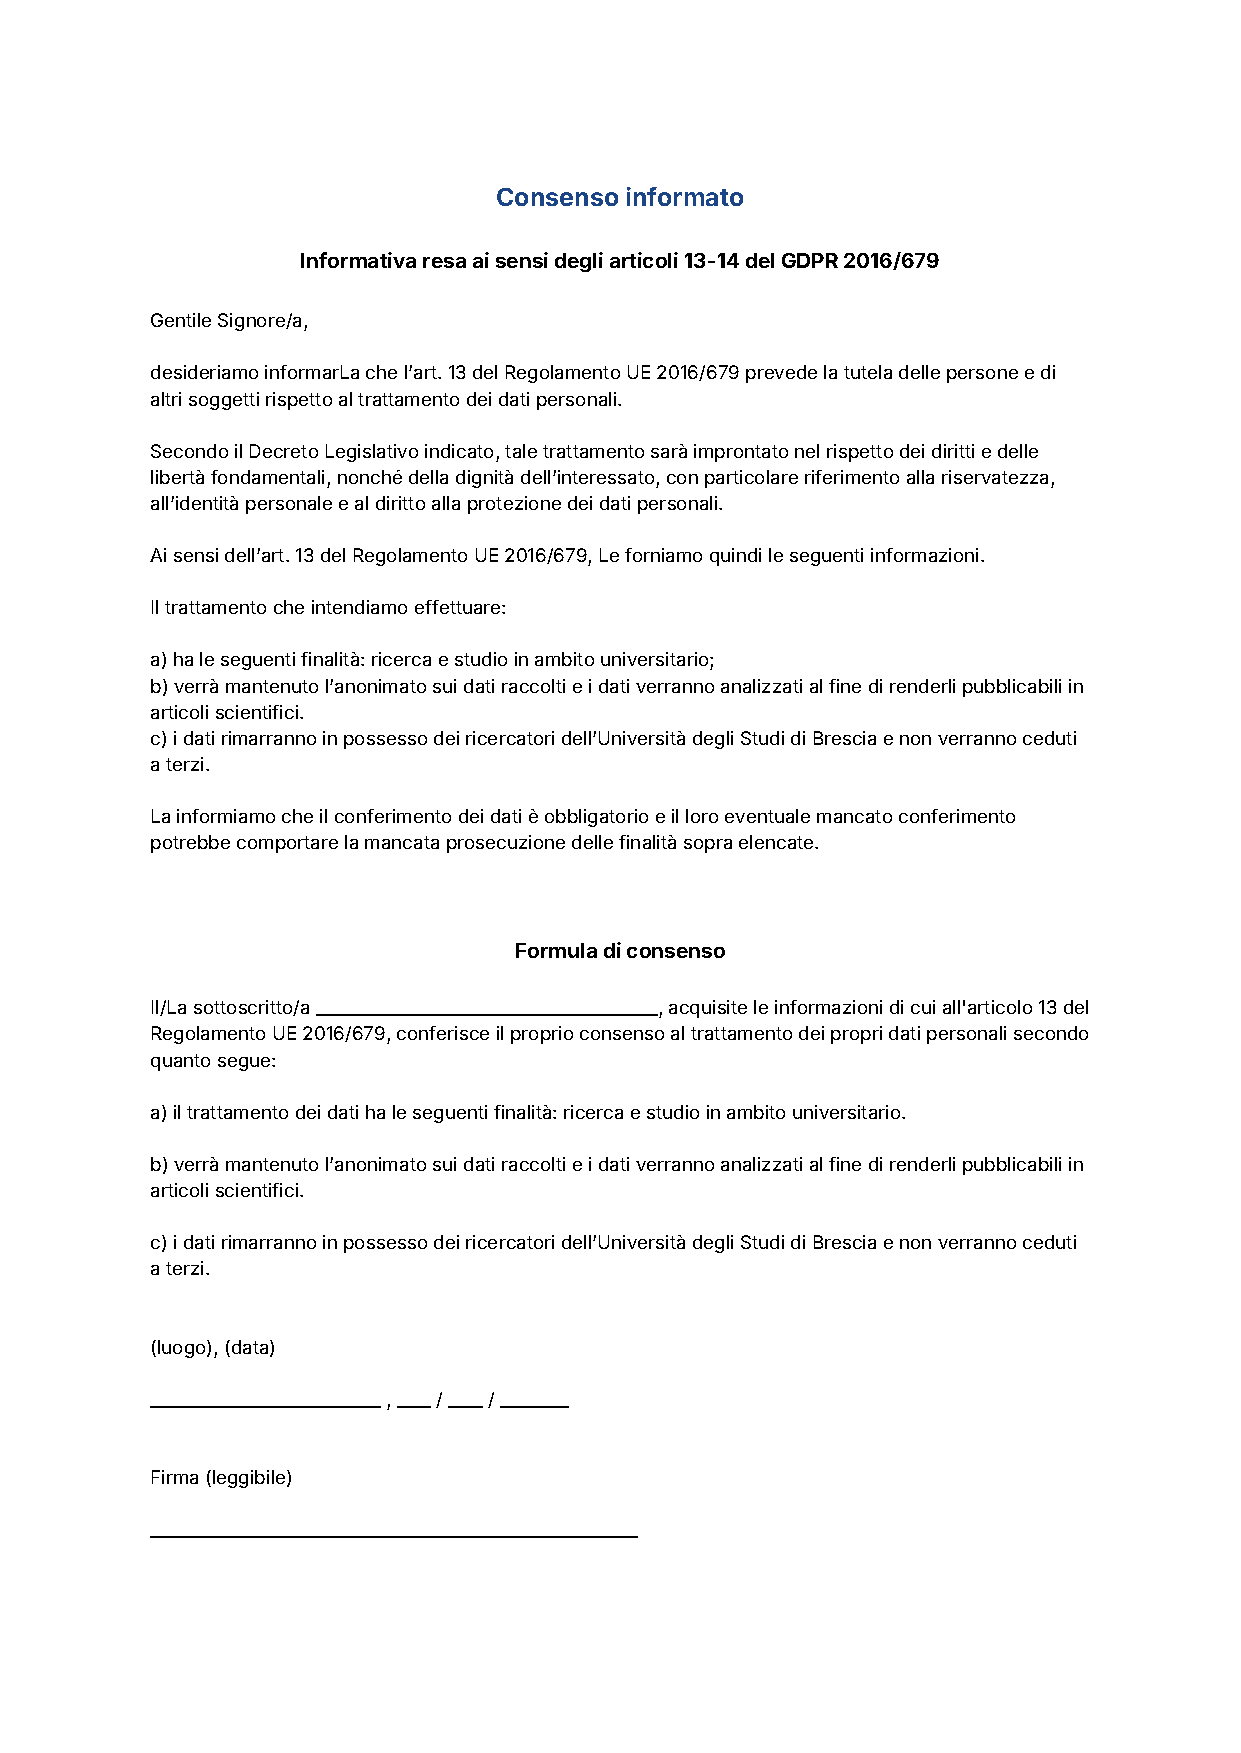
\includegraphics[width=0.8\textwidth]{./figures/05-esperimento-utenti/Consenso informato}
    \caption{Consenso informato}
    \label{fig:consenso_informato}
\end{figure}

\subsubsection{Modulo anagrafica}
\label{subsubsec:modulo_anagrafica}
A seguito dell'accettazione del modulo di consenso informato, all'utente è stato sottoposto un questionario anagrafico digitale per la raccolta dei principali dati demografici, garantendone il trattamento in forma rigorosamente anonima. Oltre alle consuete domande di inquadramento generale relative a sesso, età e titolo di studio, sono stati inseriti dei quesiti più specifici e mirati al dominio del sistema da testare. Dal momento che \textit{Brainbox} è una piattaforma rivolta agli studenti universitari per la gestione e la condivisione degli appunti, che integra strumenti basati sull'intelligenza artificiale per la trascrizione e la generazione di file audio, le domande \ref{fig:conoscenze-informatiche}, \ref{fig:uso-web}, \ref{fig:utilizzo-piattaforme} e \ref{fig:strumentiAI} sono state formulate appositamente per indagare l'esperienza e l'abitudine degli utenti con queste tematiche. Raccogliere queste informazioni di dettaglio è stato utile non solo per profilare meglio i partecipanti, ma anche per avere la possibilità, in fase di analisi dei dati, di suddividere eventualmente il campione in sottogruppi sulla base delle risposte fornite, in modo da poterne confrontare i risultati. Per i dettagli e i risultati relativi a questo tipo di indagine, si rimanda alla Sezione \ref{sec:tua_etichetta} del capitolo dedicato all'analisi dei dati.

\begin{figure}[H]
    \centering
    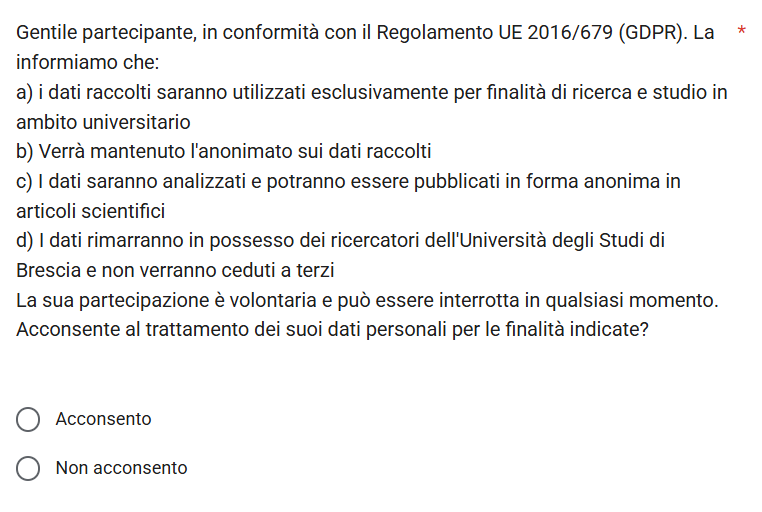
\includegraphics[width=0.8\textwidth]{./figures/05-esperimento-utenti/modulo-anagrafica/consenso.png}
    \caption{Consenso trattamento dati personali}
    \label{fig:consenso_anagrafica}
\end{figure}

\begin{figure}[H]
    \centering
    
\includegraphics[width=0.8\textwidth]{./figures/05-esperimento-utenti/modulo-anagrafica/sesso.png}
    \caption{Sesso}
    \label{fig:sesso}
\end{figure}

\begin{figure}[H]
    \centering
    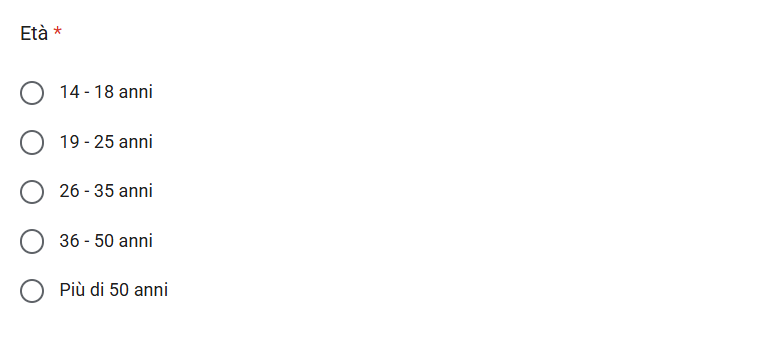
\includegraphics[width=0.8\textwidth]{./figures/05-esperimento-utenti/modulo-anagrafica/età.png}
    \caption{Età}
    \label{fig:età}
\end{figure}

\begin{figure}[H]
    \centering
    
\includegraphics[width=0.8\textwidth]{./figures/05-esperimento-utenti/modulo-anagrafica/titolo-studio.png}
    \caption{Titolo di studio}
    \label{fig:titolo-studio}
\end{figure}

\begin{figure}[H]
    \centering
    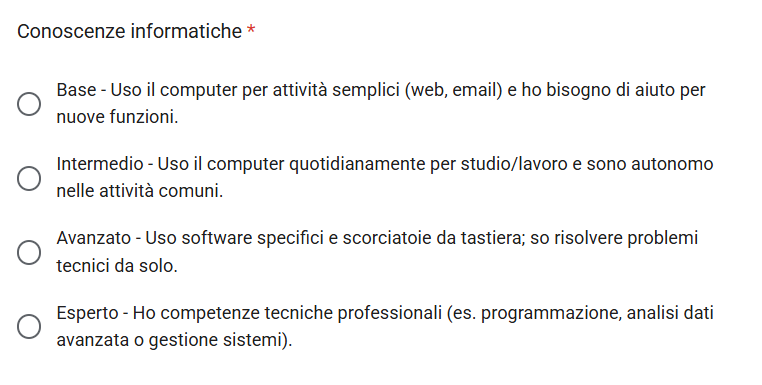
\includegraphics[width=0.8\textwidth]{./figures/05-esperimento-utenti/modulo-anagrafica/Conoscenze informatiche.png}
    \caption{Conoscenze informatiche}
    \label{fig:conoscenze-informatiche}
\end{figure}

\begin{figure}[H]
    \centering
    
\includegraphics[width=0.8\textwidth]{./figures/05-esperimento-utenti/modulo-anagrafica/uso-web.png}
    \caption{Principale uso del web}
    \label{fig:uso-web}
\end{figure}

\begin{figure}[H]
    \centering
    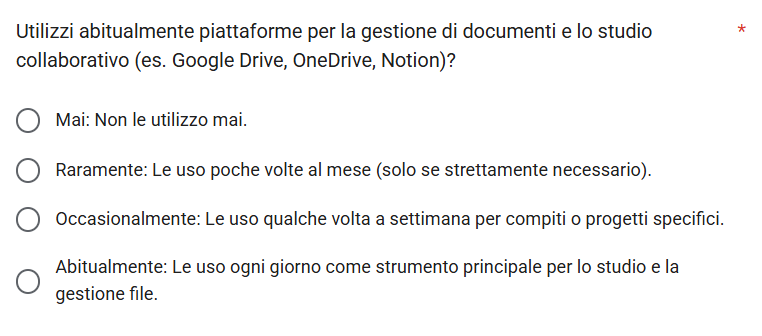
\includegraphics[width=0.8\textwidth]{./figures/05-esperimento-utenti/modulo-anagrafica/uso-ambiente-studio.png}
    \caption{Utilizzo abituale delle piattaforme di studio}
    \label{fig:utilizzo-piattaforme}
\end{figure}

\begin{figure}[H]
    \centering
    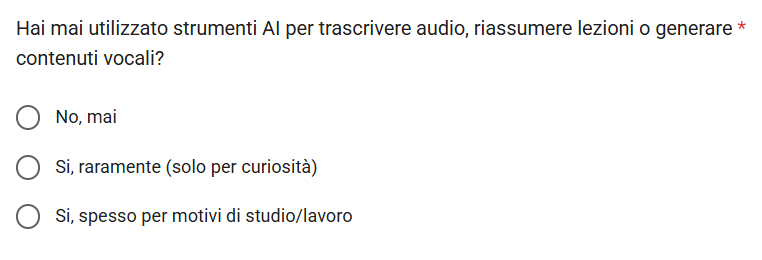
\includegraphics[width=0.8\textwidth]{./figures/05-esperimento-utenti/modulo-anagrafica/strumentiAI.png}
    \caption{Utilizzo di strumenti AI}
    \label{fig:strumentiAI}
\end{figure}

\subsubsection{Questionario di valutazione}
Terminata questa fase preliminare, l'esecuzione pratica del test è stata supportata dall'utilizzo parallelo di due ulteriori moduli, strutturati per affiancare sia il tester che l'osservatore per l'intera durata dell'esperimento. Il primo di questi è il questionario di valutazione, mantenuto aperto dall'utente durante la sessione, permetteva di leggere la descrizione dei singoli compiti (o scenari) da svolgere e di esprimere, immediatamente dopo ciascuna esecuzione, un giudizio sulla difficoltà percepita. Al termine di tutti i task, il medesimo modulo presentava il questionario SUS \textit{(System Usability Scale)} per raccogliere la valutazione complessiva dell'interfaccia (Sezione \ref{subsubsec:questionario_post_esperimento}).

\begin{figure}[H]
    \centering
    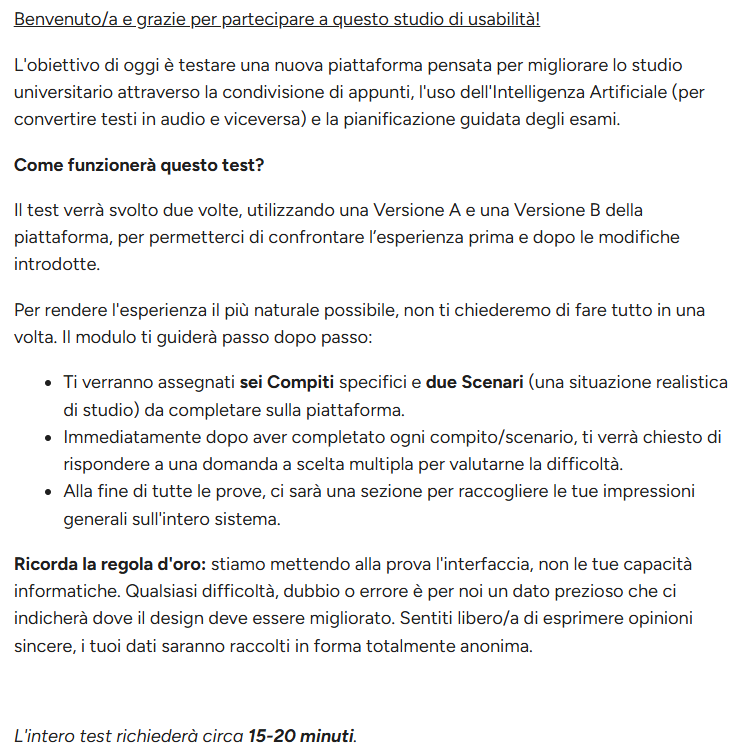
\includegraphics[width=0.8\textwidth]{./figures/05-esperimento-utenti/questionario-valutazione/benvenuto.png}
    \caption{Nota informativa}
    \label{fig:nota-informativa}
\end{figure}

Per garantire il corretto allineamento dei dati raccolti, a ogni partecipante veniva assegnato preventivamente un codice identificativo univoco da parte dello sperimentatore. L'utente doveva inserire tale codice come prima operazione all'interno del proprio modulo (come mostrato in Figura \ref{fig:id}), permettendo così di incrociare in fase di analisi le sue valutazioni soggettive con le metriche oggettive registrate dall'osservatore.

\begin{figure}[H]
    \centering
    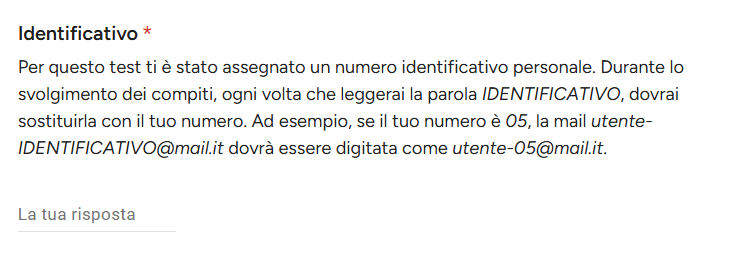
\includegraphics[width=0.8\textwidth]{./figures/05-esperimento-utenti/questionario-valutazione/identificativo.png}
    \caption{Inserimento ID utente}
    \label{fig:identificativo}
\end{figure}

Per selezionare la versione del sistema da testare (A o B), era lo sperimentatore a indicare all'utente quale opzione spuntare nel modulo. Questa scelta dipendeva dal gruppo a cui era stato assegnato il tester, in modo da alternare l'ordine di esecuzione (A-B oppure B-A) e limitare l'effetto apprendimento.

Proprio come per l'identificativo, indicare la versione corretta era fondamentale per allineare il questionario dell'utente con il modulo usato dallo sperimentatore (vedi Figura \ref{fig:vers} nella sezione relativa al modulo dello sperimentatore). Grazie a questa impostazione, è stato possibile riutilizzare gli stessi moduli per testare entrambe le versioni con ciascun partecipante: dal momento che i compiti e gli scenari erano identici per entrambe le varianti del sistema, l'utente e l'osservatore compilavano semplicemente lo stesso form prima per una versione e poi per l'altra. Questo ci ha permesso di raccogliere i dati in modo coerente e di poterli confrontare facilmente.

\begin{figure}[H]
    \centering
    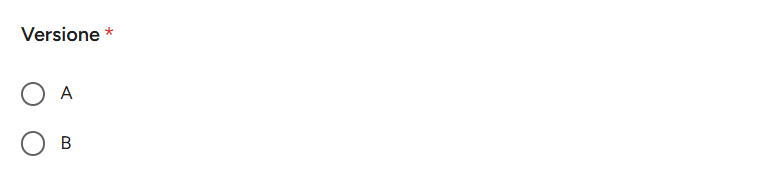
\includegraphics[width=0.8\textwidth]{./figures/05-esperimento-utenti/questionario-valutazione/versione.png}
    \caption{Selezione della versione da testare}
    \label{fig:versione}
\end{figure}

Nelle figure seguenti sono riportate le schermate del modulo relative ai sei compiti e ai due scenari proposti agli utenti. Come si può notare, al termine della descrizione di ogni task è presente una specifica domanda ("Come giudichi questo compito?" oppure "Come giudichi questo scenario?"). Per esprimere la propria valutazione, il tester ha utilizzato una \textit{scala Likert a 5 punti}, dove 1 corrispondeva a \textit{Molto facile} e 5 a \textit{Molto difficile} (passando per i valori intermedi di \textit{facile}, \textit{né facile né difficile} e \textit{difficile}). È importante precisare un dettaglio fondamentale: ai tester è stato spiegato chiaramente che il giudizio richiesto non doveva riguardare la complessità intrinseca del compito o dello scenario in sé, ma doveva misurare esclusivamente quanto l'interfaccia e il sistema ne rendessero semplice o complicata l'esecuzione.

\begin{figure}[H]
    \centering
    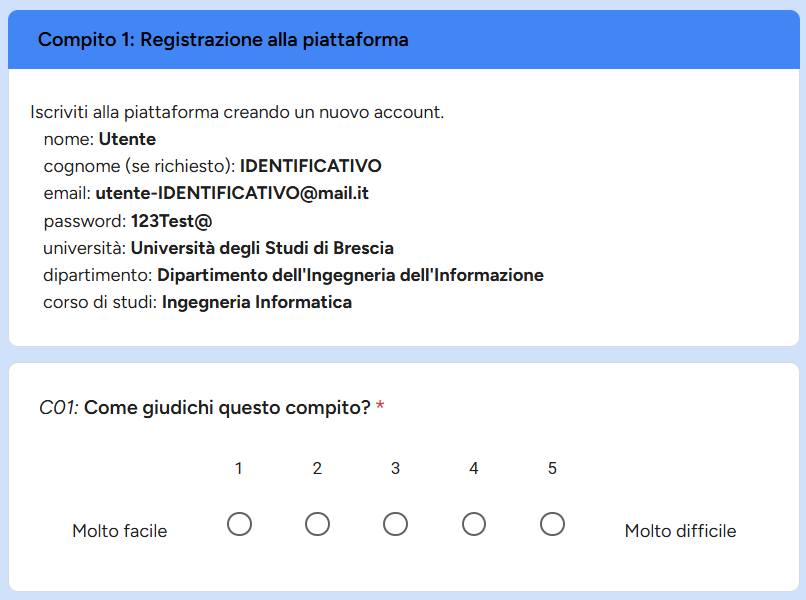
\includegraphics[width=0.8\textwidth]{./figures/05-esperimento-utenti/questionario-valutazione/compito1.png}
    \caption{Compito 1}
    \label{fig:compito1}
\end{figure}

\begin{figure}[H]
    \centering
    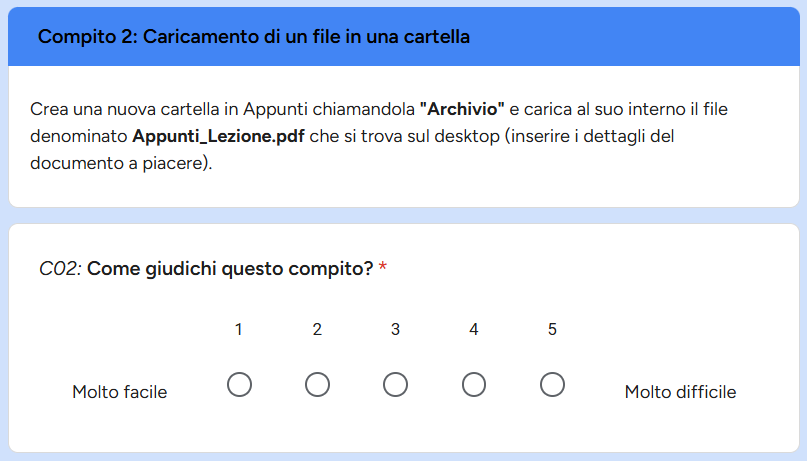
\includegraphics[width=0.8\textwidth]{./figures/05-esperimento-utenti/questionario-valutazione/compito2.png}
    \caption{Compito 2}
    \label{fig:compito2}
\end{figure}

\begin{figure}[H]
    \centering
    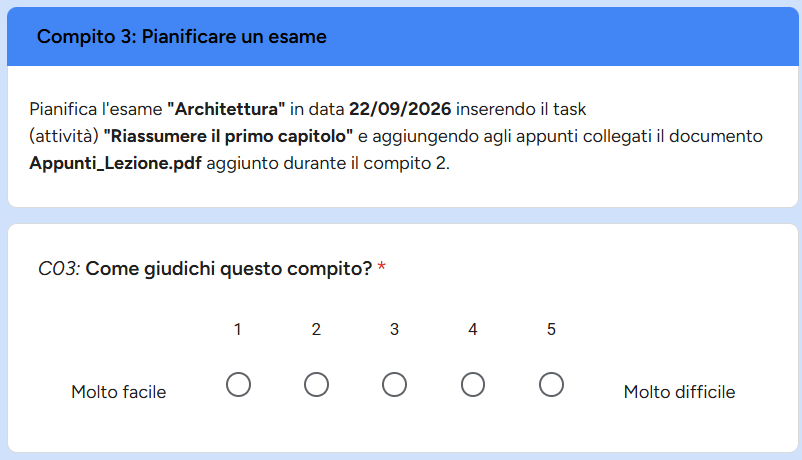
\includegraphics[width=0.8\textwidth]{./figures/05-esperimento-utenti/questionario-valutazione/compito3.png}
    \caption{Compito 3}
    \label{fig:compito3}
\end{figure}

\begin{figure}[H]
    \centering
    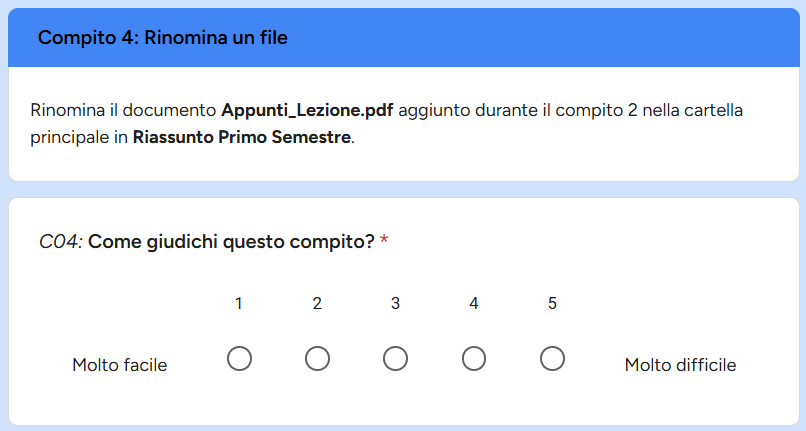
\includegraphics[width=0.8\textwidth]{./figures/05-esperimento-utenti/questionario-valutazione/compito4.png}
    \caption{Compito 4}
    \label{fig:compito4}
\end{figure}

\begin{figure}[H]
    \centering
    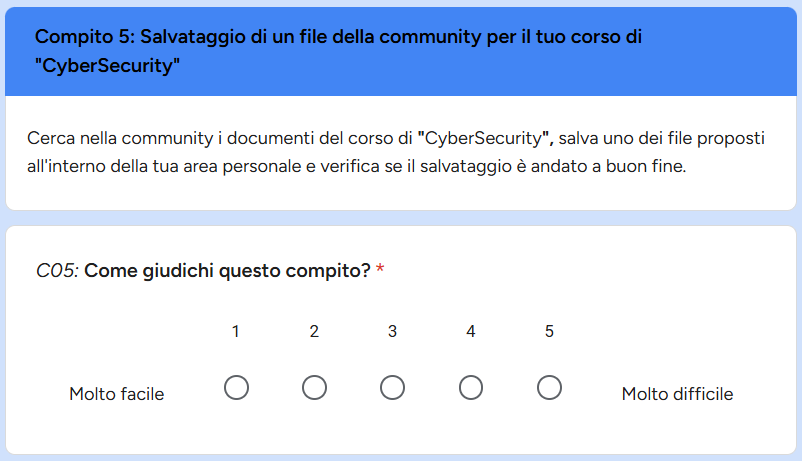
\includegraphics[width=0.8\textwidth]{./figures/05-esperimento-utenti/questionario-valutazione/compito5.png}
    \caption{Compito 5}
    \label{fig:compito5}
\end{figure}

\begin{figure}[H]
    \centering
    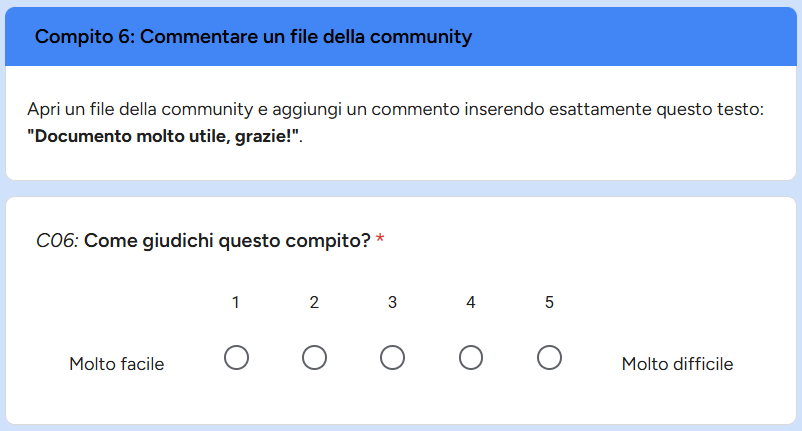
\includegraphics[width=0.8\textwidth]{./figures/05-esperimento-utenti/questionario-valutazione/compito6.png}
    \caption{Compito 6}
    \label{fig:compito6}
\end{figure}

\begin{figure}[H]
    \centering
    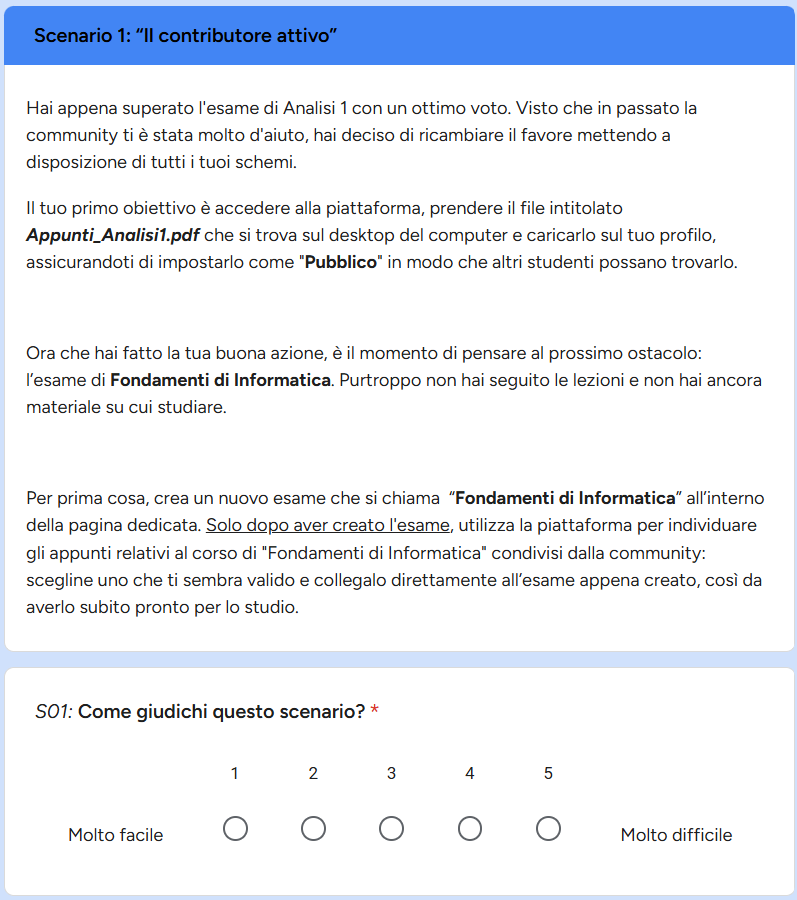
\includegraphics[width=0.8\textwidth]{./figures/05-esperimento-utenti/questionario-valutazione/scenario1.png}
    \caption{Scenario 1}
    \label{fig:scenario1}
\end{figure}

\begin{figure}[H]
    \centering
    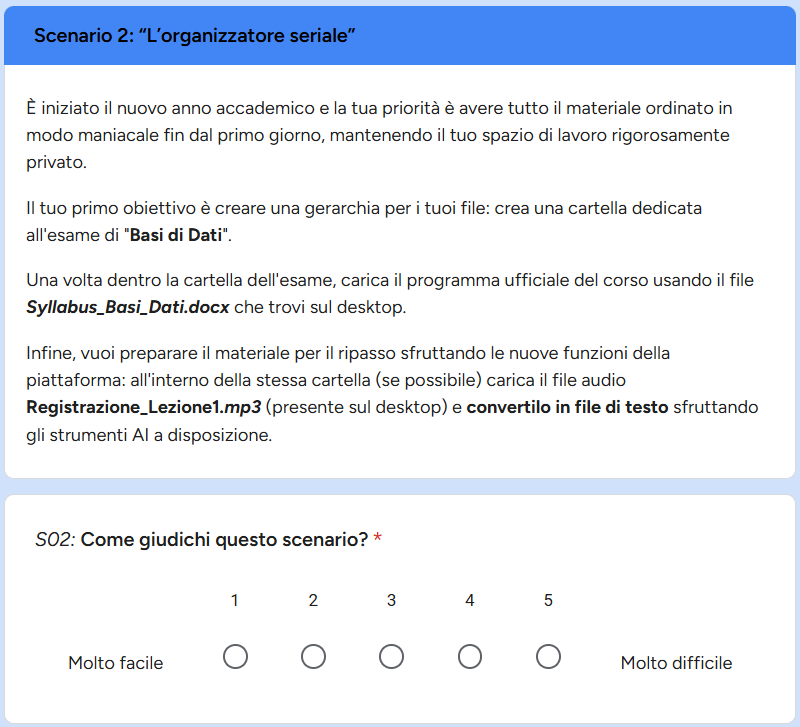
\includegraphics[width=0.8\textwidth]{./figures/05-esperimento-utenti/questionario-valutazione/scenario2.png}
    \caption{Scenario 2}
    \label{fig:scenario2}
\end{figure}

\subsubsection{Modulo per lo sperimentatore}
Come descritto in precedenza, le prime due sezioni di questo modulo (Figura \ref{fig:id} e Figura \ref{fig:vers}) riprendono esattamente l'inserimento dell'identificativo utente (Figura \ref{fig:identificativo}) e la selezione della versione (Figura \ref{fig:versione}), garantendo così il perfetto allineamento con il questionario compilato dal tester.

\begin{figure}[H]
    \centering
    
\includegraphics[width=0.8\textwidth]{./figures/05-esperimento-utenti/modulo-sperimentatore/identificativo}
    \caption{Inserimento ID utente}
    \label{fig:id}
\end{figure}

\begin{figure}[H]
    \centering
    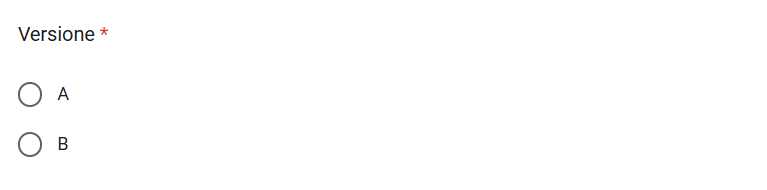
\includegraphics[width=0.8\textwidth]{./figures/05-esperimento-utenti/modulo-sperimentatore/versione}
    \caption{Selezione della versione da testare}
    \label{fig:vers}
\end{figure}

Successivamente, il modulo si struttura per singoli compiti e scenari ed è stato impiegato dall'osservatore per registrare i dati dell'esperimento. Nello specifico, la durata di esecuzione e il numero di click effettuati sono stati misurati tramite appositi tool del browser, avviati all'inizio di ogni task e azzerati prima di intraprendere quello successivo. Al termine di ciascun compito, e prima di procedere con il seguente, lo sperimentatore provvedeva ad annotare tali metriche sul modulo, integrandole con il numero di errori commessi, l'esito dell'azione, le proprie osservazioni e gli eventuali commenti espressi dall'utente.

\begin{figure}[H]
    \centering
    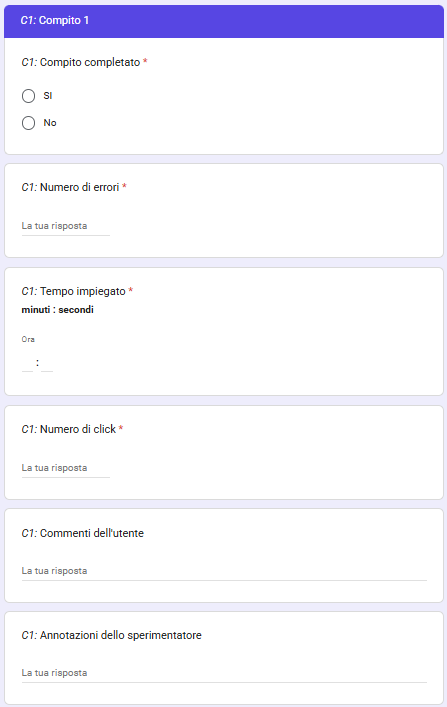
\includegraphics[width=0.7\textwidth]{./figures/05-esperimento-utenti/modulo-sperimentatore/compito1}
    \caption{Compito 1}
    \label{fig:c1}
\end{figure}

\begin{figure}[H]
    \centering
    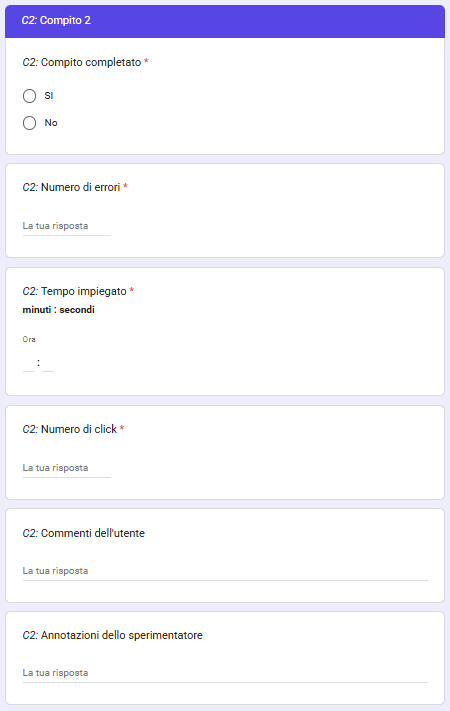
\includegraphics[width=0.7\textwidth]{./figures/05-esperimento-utenti/modulo-sperimentatore/compito2}
    \caption{Compito 2}
    \label{fig:c2}
\end{figure}

\begin{figure}[H]
    \centering
    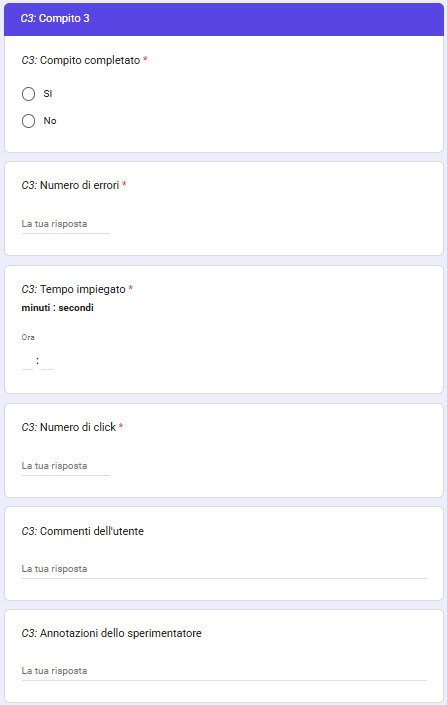
\includegraphics[width=0.7\textwidth]{./figures/05-esperimento-utenti/modulo-sperimentatore/compito3}
    \caption{Compito 3}
    \label{fig:c3}
\end{figure}

\begin{figure}[H]
    \centering
    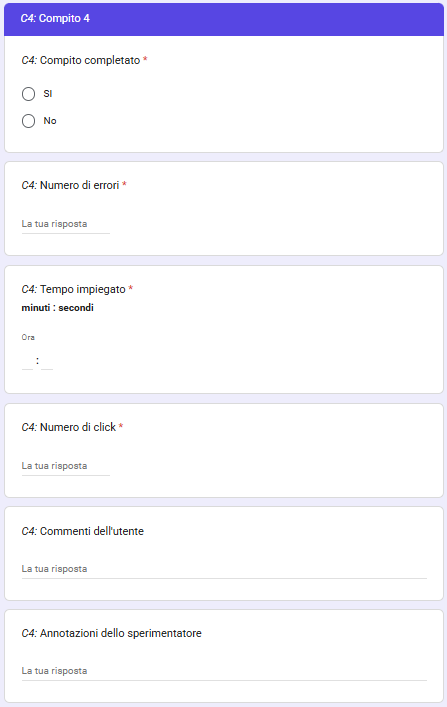
\includegraphics[width=0.7\textwidth]{./figures/05-esperimento-utenti/modulo-sperimentatore/compito4}
    \caption{Compito 4}
    \label{fig:c4}
\end{figure}

\begin{figure}[H]
    \centering
    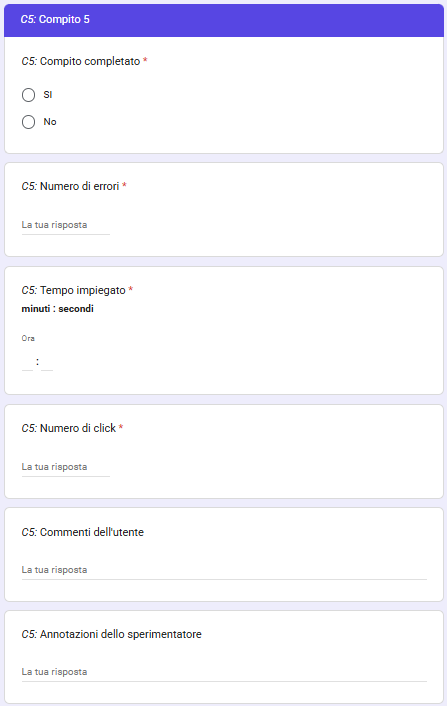
\includegraphics[width=0.7\textwidth]{./figures/05-esperimento-utenti/modulo-sperimentatore/compito5}
    \caption{Compito 5}
    \label{fig:c5}
\end{figure}

\begin{figure}[H]
    \centering
    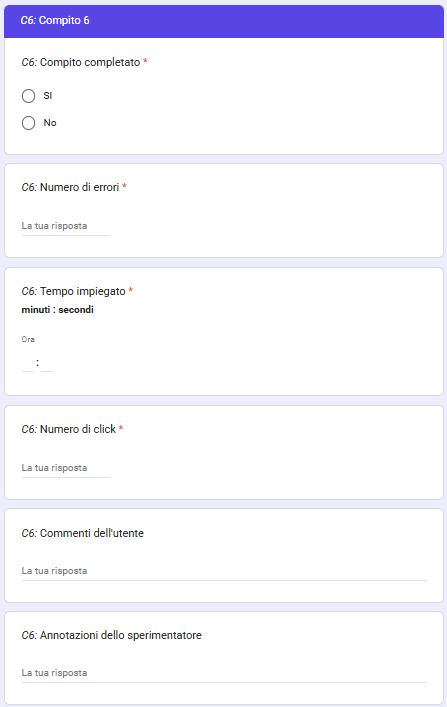
\includegraphics[width=0.7\textwidth]{./figures/05-esperimento-utenti/modulo-sperimentatore/compito6}
    \caption{Compito 6}
    \label{fig:c6}
\end{figure}

\begin{figure}[H]
    \centering
    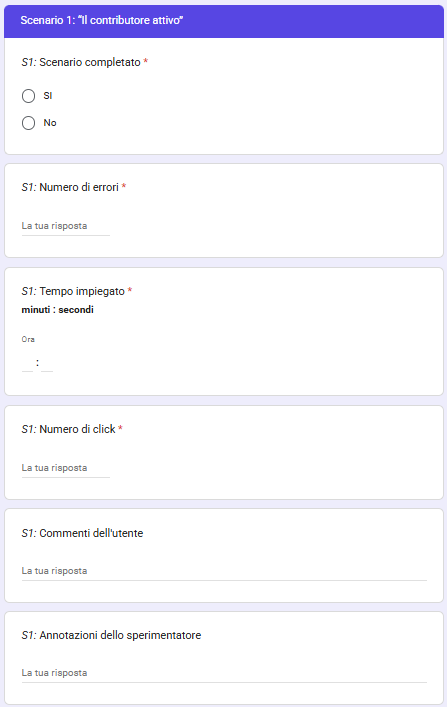
\includegraphics[width=0.7\textwidth]{./figures/05-esperimento-utenti/modulo-sperimentatore/scenario1}
    \caption{Scenario 1}
    \label{fig:s1}
\end{figure}

\begin{figure}[H]
    \centering
    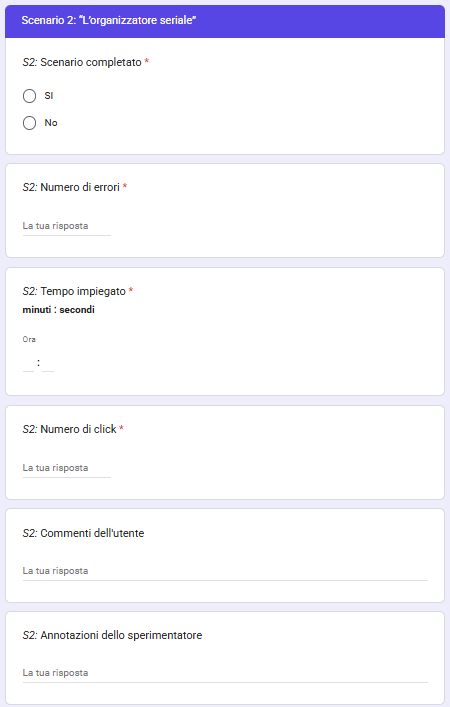
\includegraphics[width=0.7\textwidth]{./figures/05-esperimento-utenti/modulo-sperimentatore/scenario2}
    \caption{Scenario 2}
    \label{fig:s2}
\end{figure}

\subsubsection{Questionario post-esperimento}
\label{subsubsec:questionario_post_esperimento}

Al termine della sessione di test di ciascuna versione, è stato sottoposto all'utente un questionario post-esperimento per raccogliere un giudizio complessivo sull'interazione appena conclusa. Per questa fase di valutazione si è scelto di adottare il questionario SUS (\textit{System Usability Scale}), essendo uno standard ampiamente consolidato nel settore. Questo strumento propone un set di dieci affermazioni generiche e indipendenti dal dominio, rivelandosi quindi adatto a valutare qualsiasi tipologia di sistema o interfaccia. Una caratteristica peculiare del SUS è la sua struttura: per mantenere alta l'attenzione del tester ed evitare risposte meccaniche, il questionario alterna cinque affermazioni formulate in positivo a cinque formulate in negativo. Per ciascuna voce, il partecipante è chiamato a esprimere il proprio grado di accordo o disaccordo avvalendosi di una \textit{scala Likert a 5 punti} (da "Fortemente in disaccordo" a "Fortemente in accordo"). Il principale vantaggio di questo questionario risiede nella sua capacità di sintetizzare le risposte in un unico punteggio numerico: tale valore costituisce un indicatore globale dell'usabilità percepita, rendendo possibile un confronto oggettivo sia tra le due versioni testate, sia rispetto a un valore di riferimento. Per i dettagli sul metodo di calcolo effettivo del punteggio e per la relativa valutazione, si rimanda alla Sezione \ref{sec:tua_sezione_analisi}.

\begin{figure}[H]
    \centering
    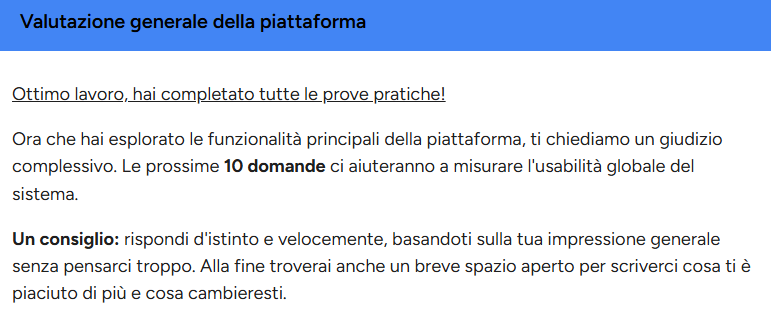
\includegraphics[width=0.8\textwidth]{./figures/05-esperimento-utenti/questionario-SUS/info-SUS.png}
    \caption{Nota informativa}
    \label{fig:info-SUS}
\end{figure}

\begin{figure}[H]
    \centering
    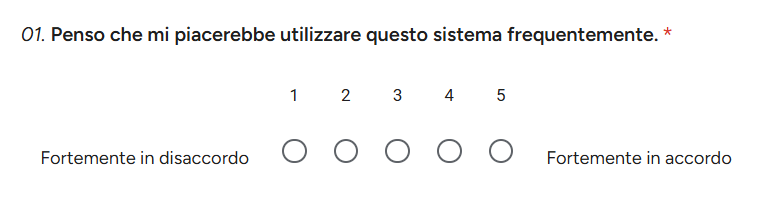
\includegraphics[width=0.8\textwidth]{./figures/05-esperimento-utenti/questionario-SUS/dom1.png}
    \caption{Affermazione 1}
    \label{fig:dom1}
\end{figure}

\begin{figure}[H]
    \centering
    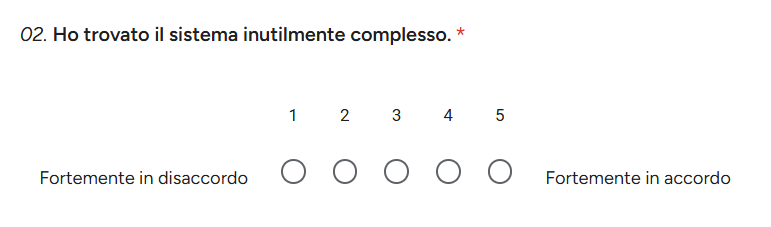
\includegraphics[width=0.8\textwidth]{./figures/05-esperimento-utenti/questionario-SUS/dom2.png}
    \caption{Affermazione 2}
    \label{fig:dom2}
\end{figure}

\begin{figure}[H]
    \centering
    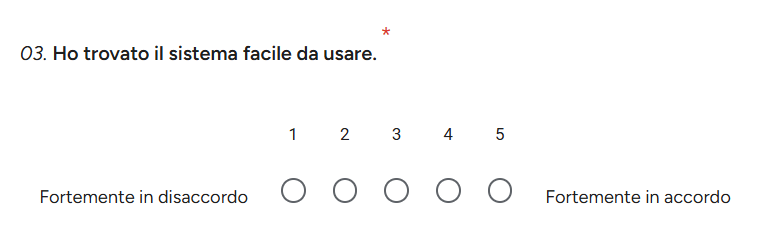
\includegraphics[width=0.8\textwidth]{./figures/05-esperimento-utenti/questionario-SUS/dom3.png}
    \caption{Affermazione 3}
    \label{fig:dom3}
\end{figure}

\begin{figure}[H]
    \centering
    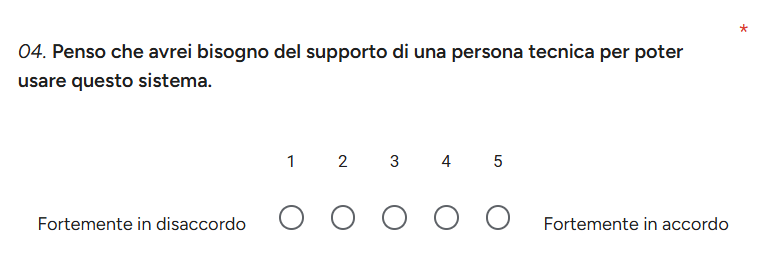
\includegraphics[width=0.8\textwidth]{./figures/05-esperimento-utenti/questionario-SUS/dom4.png}
    \caption{Affermazione 4}
    \label{fig:dom4}
\end{figure}

\begin{figure}[H]
    \centering
    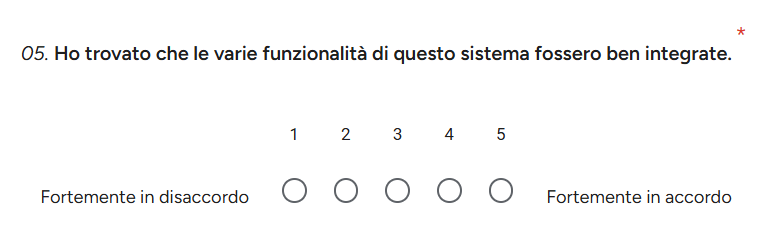
\includegraphics[width=0.8\textwidth]{./figures/05-esperimento-utenti/questionario-SUS/dom5.png}
    \caption{Affermazione 5}
    \label{fig:dom5}
\end{figure}

\begin{figure}[H]
    \centering
    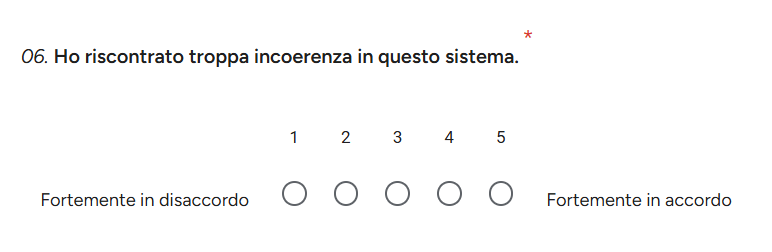
\includegraphics[width=0.8\textwidth]{./figures/05-esperimento-utenti/questionario-SUS/dom6.png}
    \caption{Affermazione 6}
    \label{fig:dom6}
\end{figure}

\begin{figure}[H]
    \centering
    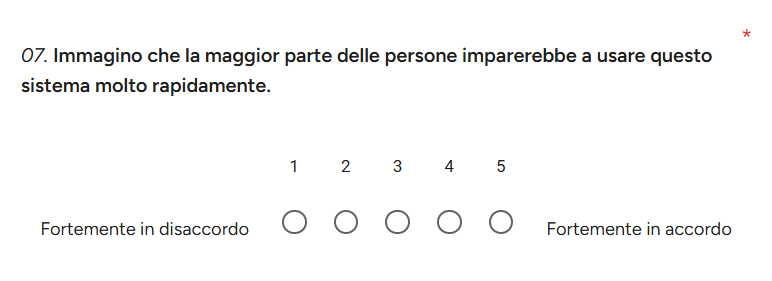
\includegraphics[width=0.8\textwidth]{./figures/05-esperimento-utenti/questionario-SUS/dom7.png}
    \caption{Affermazione 7}
    \label{fig:dom7}
\end{figure}

\begin{figure}[H]
    \centering
    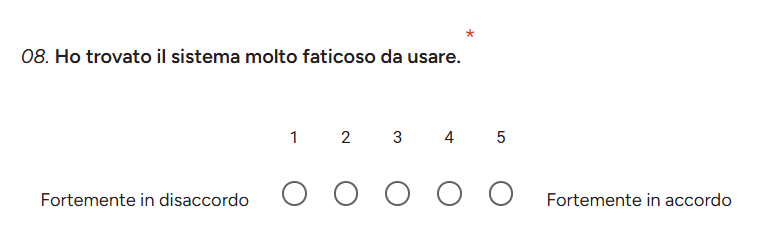
\includegraphics[width=0.8\textwidth]{./figures/05-esperimento-utenti/questionario-SUS/dom8.png}
    \caption{Affermazione 8}
    \label{fig:dom8}
\end{figure}

\begin{figure}[H]
    \centering
    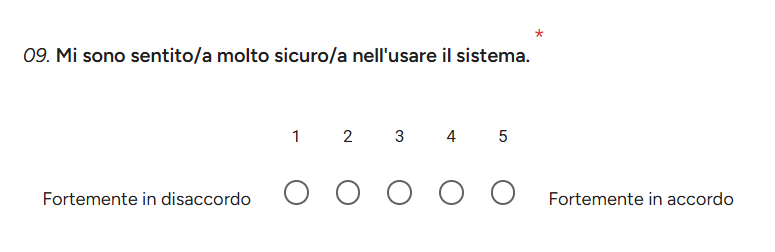
\includegraphics[width=0.8\textwidth]{./figures/05-esperimento-utenti/questionario-SUS/dom9.png}
    \caption{Affermazione 9}
    \label{fig:dom9}
\end{figure}

\begin{figure}[H]
    \centering
    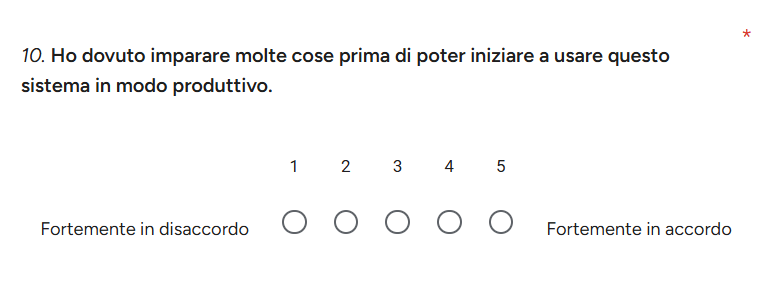
\includegraphics[width=0.8\textwidth]{./figures/05-esperimento-utenti/questionario-SUS/dom10.png}
    \caption{Affermazione 10}
    \label{fig:dom10}
\end{figure}

Infine, a chiusura del modulo, è stata predisposta un'ulteriore sezione a compilazione facoltativa (come visibile in Figura \ref{fig:impressioni}), dedicata alla raccolta di eventuali commenti, impressioni generali o suggerimenti spontanei dell'utente in merito all'intero sistema.

\begin{figure}[H]
    \centering
    
\includegraphics[width=0.8\textwidth]{./figures/05-esperimento-utenti/questionario-SUS/impressioni-generali.png}
    \caption{Inserimento impressioni generali dell'utente}
    \label{fig:impressioni}
\end{figure}

\subsubsection{Links ai moduli}
Per completezza, si riportano i collegamenti ai moduli utilizzati:
\begin{itemize}
    \item \textbf{Modulo Anagrafica:} \url{https://forms.gle/W9ce9BewdVnGAwJG8}
    \item \textbf{Questionario di valutazione:} \url{https://forms.gle/owEJTn2Dgkx1qrcp6}
    \item \textbf{Modulo per lo sperimentatore:} \url{https://forms.gle/uS6dAbXeJvTRN45d9}
\end{itemize}

\subsection{Test Pilota}
Prima di avviare ufficialmente le sessioni di test con il campione di 15 utenti, è stato condotto un \textit{test pilota} coinvolgendo un singolo partecipante esterno al progetto. Questa prova preliminare si è rivelata estremamente utile per rifinire la procedura sperimentale, chiarire la definizione delle variabili da misurare e capire esattamente come gestire e comportarsi durante lo svolgimento del test.

Nello specifico, il test pilota è servito a far emergere eventuali ambiguità od oscurità nelle istruzioni e a valutare se le richieste dei compiti e degli scenari fossero chiare e di immediata comprensione per l'utente. Inoltre, ha permesso di verificare in modo pratico la durata dell'intero esperimento e delle singole prove, assicurandosi che i compiti non fossero troppo difficili e i tempi troppo stretti o, al contrario, eccessivamente lunghi.

Proprio grazie a questa prova generale, è stato notato che le tempistiche risultavano un po' lunghe e sono state individuate alcune incomprensioni pratiche, legate soprattutto alla formulazione dei due scenari. Sulla base di questi riscontri, le tracce e le richieste sono state ricalibrate e aggiustate, garantendo così la massima fluidità e l'assenza di intoppi durante le sessioni di test definitive.